\documentclass{article}
\usepackage{ctex}
\usepackage{amsmath}
\usepackage{booktabs}
\usepackage{graphicx}
\usepackage{caption}
\usepackage{multirow}
\usepackage{geometry}
\usepackage{subfigure}
\usepackage{cite}
\geometry{a4paper}
\geometry{left=1cm}
\geometry{right=1cm}
\begin{document}
\title{一种基于DBSCAN的过采样方法
Multi-category oversampling based on DBSCAN and Gaussian distributions}
\author{肖一诺}
\bibliographystyle{plain} 
\maketitle
%hello,world
%肖一诺 \cite{2020Combined}
%一定会成功
\section{Abstract}
在不平衡数据集上进行分类学习是机器学习分类任务中最具挑战性的任务之一。
因为在不平衡数据集中,数据的分布不平衡导致对于少数类数据的预测能力较差。
不平衡问题根据类别的多少又可分为多类别和二分类不平衡问题。
多类别的不平衡问题类之间的关系要比二分类问题复杂,
多类别问题中可能存在一个多数类,几个少数类,也可能存在几个多数类,
几个少数类,甚至一个类别相对于某些类别是多数类,相对于其他类别又成了少数类,
如何解决多类别分类问题同样是需要解决的问题。目前已经提出了很多可取的过采样方法,
比如说$SMOTE$和基于$SMOTE$的一些方法。
这些方法能在一定程度上应对不平衡数据的问题,
但是这些方法无法有效处理成簇的数据,并且在过采样的过程中,
容易产生数据覆盖的问题,而且$SMOTE$的方法容易受到噪声点的影响。
针对这些问题,我们提出了一种新的过采样方法,该方法结合了多种方法,
如DBSCAN聚簇数据,利用高斯分布拟合数据并生成新的数据,对多数类样本进行清洗等。
该方法适用于二分类和多分类问题,能够有效地拟合分簇的数据进而生成数据,
并且该方法对噪声数据不敏感而且能够减轻数据覆盖。实验表明,
$DB-OGC$算法在多种评价指标上要好于现有的过采样方法。

\section{Introduction}
不平衡数据指的是那些不同类别之间的数据量并不均衡的数据集。
不平衡数据集在现实中的很多应用领域中都很常见,
比如说医疗诊断,欺诈检测等等。医疗诊断中患病样本是少数类样本,
欺诈检测中欺诈样本为少数类样本。我们往往对数据集中的少数类样本感兴趣,
因为少数类样本往往包含有更多的价值。但是由于数据集是不平衡的,
现有的机器学习模型都会在预测的过程中使得预测结果偏向于多数类类别,
进而忽视少数类类别。\cite{2016A}因此我们需要对不平衡数据集进行特殊处理来达到更好地预测的目的。
处理不平衡数据集的方法大概可以分为算法层面和数据层面两种类型。基于算法的方法尝试提出新的模型用于解决不平衡数据预测问题,
而数据层面的方法尝试改变数据的分布,使数据达到平衡。基于算法的方法又大致上可以分为cost-sensitive的方法\cite{article,2010Risk}或者是集成(ensemble)方法。
cost-sensitive方法更改权重或者损失提高分类器的性能\cite{2007Highcost-sensitive},adaboost\cite{10.1007/3-540-59119-2_166}是一种提升算法,前一个错误分类的少数类样本的权值会逐渐增大。
集成分类器为多分类系统,通过将一组基本的分类器组合到一起,
改进了整体分类器的学习结果。ensemble方法又大致上可以分为Boosting\cite{article_boosting}方法和Bagging\cite{2018Multi}方法。
Boosting方法有SMOTEBoost\cite{2003SMOTEBoost},XGBoost\cite{Chen_2016},等等。在Adaboost\cite{10.1007/3-540-59119-2_166}算法中同样融入了Boosting的思想。但是基于算法的解决方法局限于单一类型的分类器。

%二分类和多分类
现有的过采样方法可能在二分类问题中有不错的表现,但是在多分类问题上表现欠佳。在二分类问题上,
确定两个类之间的关系比较简单,但是在多分类问题上类之间的关系要复杂的多。
很多现有的处理两种类别的方法无法直接有效处理位于多个类别边界的样本点,容易产生ovelapping。现有处理多分类的问题
可以将多分类问题转化成两两二分类问题,但是这样的话单独处理某两个类时会忽视掉其余类别样本
因此我们设计的方法需要能够在处理某个类别的样本时考虑到其余不同类别样本。


%介绍基于data的smote方法
相对于基于算法的处理不平衡数据集的方法,基于数据的方法通过改变数据分布使得数据集适合于一般性的机器学习算法。
我们可以通过降采样,或者过采样方法重构数据分布。
其中最为经典的过采样方法为$SMOTE$\cite{2002SMOTE}算法。$SMOTE$为一种基于随机过采样算法的改进方法,通过在少数类样本点的连线上随机生成新的样本点的方法实现过采样。
同时还有许多基于$SMOTE$的改进方法,比如说$Boardline-SMOTE$\cite{2005Borderline}算法,
$ADASYN$\cite{2008ADASYN}算法等。Boardline-SMOTE算法着重看中位于”边界“区域的少数类样本点,
$ADASYN$算法为一种自适应的算法,该算法自适应计算每个少数类样本周围应该合成样本点的数量。
然而这些算法同样存在一些问题。基于$SMOTE$的算法容易受到噪声点的影响\cite{2017CCR}.
在噪声点附近生成数据容易产生overlapping现象,生成的少数类样本点和多数类
样本点区域覆盖,影响决策的过程。除了噪声点,$SMOTE$的方法对分簇的数据处理同样较差。
如果某一类少数类样本点的分布于多个簇中,$SMOTE$则算法无法捕捉到簇状分布。
另外,在利用$SMOTE$等方法生成新的数据后,原有的少数类样本点的数据分布可能发生了变化,会影响到数据的预测。

%解释一下聚类算法
聚类算法能够处理簇形数据,我们可以想利用聚类算法将统一类别的数据划分到多个簇当中,针对每一个簇我们对其进行过采样。聚类算法有很多种,其中最知名的为
$K-means$算法。但是$K-means$算法为基于距离的算法,当出现不规则的簇时$K-means$算法难以处理,并且$K-means$的超参数K难以设置。因此我们采用基于密度的
$DBSCAN$算法。


%提出新的方法
针对这些问题,我们提出了$MC-ODG$算法,该算法能够有效处理簇形数据,并且不易受到噪声点的影响且不易产生overlapping现象,生成的数据保留原有的数据分布。
$MC-ODG$算法应用到了$DBSCAN$聚类方法和高斯分布拟合数据。在多个实验数据集的多个指标上,我们提出的$MC-ODG$算法要优于现有的方法。

我们提出的$MC-ODG$算法的贡献如下:
\begin{itemize}
  \item $MC-ODG$提出了一种可以有效处理分簇数据的过采样方法。
  \item $MC-ODG$解释了噪声数据点会对过采样过程产生什么影响,给出了如何处理噪声数据点的方法。
  \item $MC-ODG$提出了一种在过采样后能够保留原有数据分布的方法。
  \item $MC-ODG$不仅适用于二分类问题,可以推广到多分类问题,能够充分利用多个类别之间的分布信息。
\end{itemize}


\section{相关工作}


\section{MC-ODG Algorithm}
该部分将详细介绍$MC-ODG$算法。之前提到基于$SMOTE$的各种方法,不能有效处理噪声点和分簇的数据。
如果数据中存在噪声,生成新的数据之后可能会产生$overlpping$现象。同时,
基于$SMOTE$的方法生成的数据点不能够保留原有数据的分布。同样,$MC-CCR$方法是在某个范围内随机生成部分数据点,
没有保留原有少数类样本点的分布。同时$MC-CCR$方法可能会在噪声类样本点附近生成过多的对应少数类别样本,
会对预测结果产生不良影响。针对上述方法的多种缺点,我们提出了$MC-ODG$方法,避免出现上面提到的诸多问题。
\subsection{二分类问题}
我们首先给出$ODG$算法,该算法用于解决二分类不平衡问题。
\subsubsection{利用$DBSCAN$算法划分少数类样本点}
不平衡数据集中样本点分为多数类样本点和少数类样本点。
我们需要首先利用$DBSCAN$算法对少数类样本点进行划分。
经过$DBSCAN$划分后,该少数类样本点被划分为核心点,边界点和噪声点。少数类样本点可能存在一个簇,也可能存在多个簇。
接下来我们需要分别地在核心点,边界点和噪声点附近生成新的数据,已达到过采样的目的。
在这里我们假设多数类样本点的数量为$N_{maj}$,少数数类样本点的数量为$N_{min}$,那么我们可以得到过采样的样本量公式 \ref{equation1}:
\begin{equation}\label{equation1}
  N_{oversampling}=N_{maj}-N_{min}
\end{equation}
在得到总的过采样样本数量后,我们需要确定在核心点,边界点和噪声点上生成样本点的比例。首选需要确定的是除非
无法在少数类样本点上形有效聚簇的情况下,不在噪声类样本点附近生成样本点。无法形成有效聚簇也就是指经过$DBSCAN$算法后,绝大部分样本点均
标记为噪声类样本点,这种情况我们特殊处理。在一般情况下,我们记边界点上生成新的样本点比例为$\alpha$,
那么很容易得到边界点上和核心点上生成样本量的数量$N_{boardline}$和$N_{core}$在公式\ref{equation2}中:
\begin{equation}
  \label{equation2}
\begin{aligned}
  N_{boardline}=N_{oversampling}\times \alpha \\
  N_{core}=N_{oversampling}-N_{boardline}
\end{aligned}
\end{equation}

\begin{figure}
  \centering
  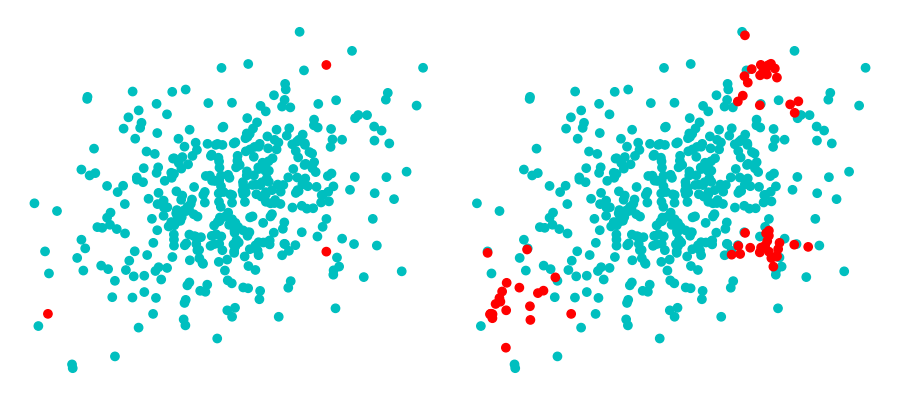
\includegraphics[width=.8\textwidth]{myplot1.png}
  \caption{$\alpha$随边界点比例变化}
  \label{fig1}
\end{figure}
参数$\alpha$的可以通过超参数来指定,同时也可以根据边界点和核心点的比例自适应确定。一般情况下,$\alpha$的值大于边界点在样本点中的比例。
因为我们更加偏向于在边界点生成数据,使得分类面偏向于少数类样本点。因此得到$\alpha$和$N_{outline}$和$N_{min}$的关系如图 \ref {fig1}所示:
\subsubsection{在边界点上生成数据}
接下来介绍在边界点处生成新的数据的方法。每个边界点都对应于某个簇,而这个簇的中心点最能够代表该簇数据的分布。
我们可以计算出簇中心点的对应的协方差矩阵,对其进行缩放后利用高斯分布在对应边界点处生成样本点。
我们记该边界点为$point$,函数$cov$为计算协方差矩阵的函数,$core\_points$为核心点构成的矩阵,核心点数量为$num\_core\_points$,$n_{boardline}$为在该边界点附近生成新样本数量,
利用高斯分布生成新的样本点的函数为$multivariate\_normal$,则得到新的样本点$new\_data$的公式为 \ref{equation3}:
\begin{equation}
  \label{equation3}
  \begin{aligned}
     & cov\_mat=cov(core\_points)/num\_core\_points \\
     & new\_data=multivariate\_normal(point,cov\_mat,n_{boardline})
  \end{aligned}
\end{equation}
我们还需要确定在特定的边界点生成新的样本的的数量$n_{boardline}$。为了提高机器学习算法预测少数类样本点的能力,
我们希望在少数类和多数类的边界附近生成较多的少数类样本点,以此使得决策边界向少数类样本点靠拢。
我们计算每个边界样本点的$k$近邻,如果说少数类样本点的$k$近邻中多数类样本点较多,说明改点更加靠近两类点的决策边界,
在该点附近生成的样本点也就越多。
我们记该点$k$近邻中多数类样本点数量为$n\_knearest\_maj$,可以得到$n_{boardline}$的计算公式为 \ref{equation4}:
\begin{equation}
  \label{equation4}
  n=\frac{n\_knearest\_maj}{\sum_{i\in minority} n\_knearest\_maj}\times N_{boardline}
\end{equation}
在得到某个边界点附近生成样本点数量$n_{boardline}$后,我们还需要限制$n_{boardline}$的最大值,避免在单个样本点附近生成过多的少数类样本。因为有的数据集
在训练过程中可能存在极端分布,在某个样本点附近生成过多少数类样本点,
从而改变了原有数据的分布,对模型的训练产生不良影响。我们通过限制$N_{boardline}$的最大值控制单个样本点生成数量解决这个问题。我们定义参数$multiple\_k$,
限制生成样本点数量最大值为$multiple\_k\times k$,如公式 \ref{equation5}所示:
\begin{equation}
  \label{equation5}
  N_{boardline}=min(multiple\_k \times k, N_{boardline})
\end{equation}
\begin{figure}
  \centering
  \includegraphics[width=.8\textwidth]{myplot2.png}
  \caption{最左端图为原始样本点,中间图为在没有限制单个样本点生成数量情况下得到的数据分布,最右端为限制了单个样本点生成数量情况下的过采样结果}
  \label{fig2}
\end{figure}
在图\ref{fig2}中,最左端图为数据原始分布,中间图为在没有限制单个样本点生成数量情况下得到的数据分布,
最右端为限制了单个样本点生成数量情况下的过采样结果。我们可以发现在图右下方某个样本点处生成了过多的样本点
,从而影响了少数类样本点的整体分布。显然右图更符合原始数据的分布情况。
\subsubsection{在核心点上生成新的样本点}
我们通过$DBSCAN$算法将样本点分成多个簇,在每个簇的核心点上生成新样本点数量取决于该簇中样本点的数量大小。我们记该簇上样本点数量为$num\_data\_cluster$,
我们可以得到单个簇上样本点生成数量$n_{core}$,如公式\ref{equation6}所示。
\begin{equation}
  \label{equation6}
  n_{core}=\frac{num\_data\_cluster}{\sum_{i \in cluster} num\_data\_cluster}
\end{equation}
生成方法和边界点处生成方法类似,假设单个簇中样本点的分布服从高斯分布,利用核心点的均值和方差生成新的样本点。我们令$mean$函数为取均值函数,得到
在核心点上生成新样本的公式\ref{equation7}。
\begin{equation}
  \label{equation7}
  \begin{aligned}
    & cov\_mat=cov(core\_points) \\
    & new\_data=multivariate\_normal(mean(core\_points),cov_mat,n_{core})
  \end{aligned}
\end{equation}

\subsubsection{在噪声点上生成新的样本点}
%这里需要添加部分实验证明
一般情况下不会在噪声点上生成新的样本点,只有当该类型少数类样本点无法形成有效聚簇时,
即大部分该类型样本点均标记为噪声点时,噪声点比例$radio$超过某个超参数$noise\_radio$(一般设置为0.5)时,才会在噪声点处生成部分新样本。
随着噪声类样本点数据量的增加,在噪声点上生成数据的比例同样增加。在噪声点处生成新的样本所占总生成样本比例$\alpha$的公式\ref{equation10}:
\begin{equation}
  \label{equation10}
  \alpha=\frac{0.9}{1-{noise\_raodio}^2}\times radio^2+1-\frac{0.9}{1-{noise\_raodio}^2}
\end{equation}
和在边界点处的处理相同,我们需要限制在单个噪声点处生成的样本点数量,最终生成数量$N_{noise}$公式为\ref{equation11}。
\begin{equation}
  \label{equation11}
  \begin{aligned}
   &  N_{noise}=\alpha \times N_{oversampling} \\
   & N_{noise}=min(multiple\_k \times k, N_{noise})
  \end{aligned}
\end{equation}
在计算完噪声点附近生成样本点数量后,再根据比例计算需要在边界点和核心点生成样本点数量。采用如上的公式原因在于当噪声点比例正好为
超参数$noise\_radio$时,生成比例为$0.1$。当$noise\_radio$大致为0.5时,函数图像为图\ref{fig4}。
\begin{figure}
  \centering
  \includegraphics[width=.8\textwidth]{myplot4.png}
  \caption{左图中少数类样本过于稀少而且距离较远,不能够形成有效聚簇。利用在噪声点附近生成样本点的方法,经过过采样后如右图所示}
  \label{fig4}
\end{figure}
%由于该类型样本点数量过少,
%如果生成过多样本点虽然会
%提升对少数类样本点的预测能力,但是很有可能会影响到其余样本点的预测。此时我们需要重新
%确定生成样本点的数量,可以利用公式\ref{equation8}得到新的样本点数量$N_{oversampling}$,其中$rate$为超参数,一般默认为5。
%\begin{equation}
%  \label{equation8}
%  N_{oversampling}=(N_{maj}-N_{min})/rate
%\end{equation}
由于无法生成有效聚簇因此无法利用高斯分布生成数据。在这里采样$SMOTE$算法中的方法,
每次生成样本点时从该样本点的$k$近邻样本点中随机选择单个样本,在两个点之间的连线上随机生成样本点。
我们令$\gamma$为$0-1$之间的随机数,少数类样本点和$k$近邻中选中的样本点分别为$point1$和$point2$,则生成新样本点的公式\ref{equation9}。
\begin{equation}
  \label{equation9}
  new\_point=point1+\gamma \times (point2-point1)
\end{equation}
\begin{figure}
  \centering
  \includegraphics[width=.8\textwidth]{myplot3.png}
  \caption{左图中少数类样本过于稀少而且距离较远,不能够形成有效聚簇。利用在噪声点附近生成样本点的方法,经过过采样后如右图所示}
  \label{fig3}
\end{figure}
如图\ref{fig3}所示,\ref{fig3}中左图为原始数据分布,其中少数类样本点数量过于稀少,无法形成有效聚簇。这时无法在边界点和核心点处生成数据,采用在噪声点附近生成数据的方法。
经过过采样后的结果如\ref{fig3}右图所示。


\subsubsection{多数类样本点的平移}
根据少数类样本点的分布特征我们需要生成部分数据。同时我们也对少数类样本点附近的多数类样本点进行部分处理。在\cite{2017CCR}中给出了
CCR模型,该模型采用了一种cleaning的方法来处理部分多数类样本点。
CCR在每个少数类样本点周围画出一个圆形区域(二维空间上),并将圆形区域内部的
多数类样本点移出到圆形区域之外。在$MC-ODG$方法中同样可以利用相似的方法。在处理边界点时计算了每个少数类样本的$k$近邻,以该样本点为中心,
$k$近邻中最大距离为半径画
出一个区域,我们可以将这些$k$近邻中的
多数类样本点移出该区域。

\subsubsection{复杂度分析}
在这里我们给出处理二分类问题的过采样方法$ODG$的时间复杂度。
我们假设二分类问题中多数类样本数量为$N_{maj}$,少数类样本数量为$N_{min}$,总的样本数为$N$,数据集上属性的个数为$m$。
在$DBSCAN$算法过程中,时间复杂度可以控制在$O(mN_{min}\log(N_{min})$,上限为$O(mNlog(N))$。在计算少数类样本点的$K$近邻时,该步骤的时间复杂度为
$O(mN_{min}N+N_{min}Nlog(N))$,上限为$O(mN^2)$。因此这一步的时间复杂度可以表示为$O(mN(N+log(N)))$。


\subsection{多分类问题}
多分类不平衡问题要比二分类不平衡问题更加难以解决。在二分类问题中,很容易区分出多数类别和少数类别。
但是在多分类问题中,类别之间的关系更加复杂,难以处理。
多个类别中,多数类别和少数类别都有可能存在多个,
一个类别相对于某个类别可能是多数类,但是相对于其他类别可能会当做少数类。
多类别问题中,overlapping和noise的问题也会更加严重。现有的处理多分类问题的方法可以大致上分为OVA和OVO两种。
我们假设存在m个类别,OVA问题将多分类问题转化为m个二分类问题,每个单独问题中取出某一类,其余类别作为另一个类别。
OVO则是需要训练$m(m-1)/2$个二分类器,每两个类别之间训练一个分类器。这两种处理方法都存在各自的问题。OVA方法中忽视了合并成统一类别的各个类别之间的信息,
随着类别数量的增加,OVO方法的复杂度也随之快速增大。
在\cite{2017CCR,2019Radial}中给出了一种处理多分类问题的方法。我们对多个类别迭代处理。我们对每个类别进行过采样时,
在已经处理好的类别中选出一个子集作为多数类,该类别作为少数类,利用二分类的过采样方法处理。我们先将多个类别按照样本数量倒序排列,针对每个少数类别,从已经处理过的
多数类别中选择一个子集,利用$ODG$算法处理后,将该少数类别标记为多数类别。

\subsubsection{复杂度分析}
同样我们总的样本数为$N$,数据集上属性的个数为$m$,同时令类别的个数为$c$。我们相当于是做了$c-1$次针对二分类数据集的过采样,时间复杂度可以表示为
$O(cmN(N+log(N)))$。

\section{实验}
在本章节中,我们会详细介绍针对$ODG$和$MC-ODG$所进行的一系列实验。我们将$MC-ODG$算法和现有的,比较成熟的
过采样方法进行比较,我们发现在多个不同的指标上,我们的基于$ODG$的算法能够取得更好的结果。

\subsection{评估指标}
我们在多个指标上评估不同的过采样方法。在不平衡数据集上,预测准确度不是评级模型预测结果的良好指标。由于数据不平衡,准确度指标会自然
偏向多数类类别数据。
\subsubsection{二分类问题}
我们在此令多数类样本的标签为0(Negative),少数类样本的标签为1(Positive)。
$Precision$,$Recall$,$F-value$和$auc$值是更加合理的评测指标。表\ref{table1}给出了二分类问题的混淆矩阵。
% Please add the following required packages to your document preamble:
% \usepackage{booktabs}
\begin{table}[]
  \caption{Confusion matrix for the two-class problem}
  \label{table1}
  \begin{tabular}{@{}ccc@{}}
  \toprule
  Actual label & \multicolumn{1}{l}{Predicted positive} & \multicolumn{1}{l}{Predicted negative} \\ \midrule
  Positive     & TP                                     & FN                                     \\
  Negative     & FP                                     & FN                                     \\ \bottomrule
  \end{tabular}
  \end{table}
利用该混淆矩阵我们可以计算出Precision,Recall和F-value。计算公式分别如下:
\begin{equation}
  Precision=\frac{TP}{TP+FP}
\end{equation}
\begin{equation}
  Recall=\frac{TP}{TP+FN}
\end{equation}
\begin{equation}
  F-value=\frac{(1+\beta^2) \times Precision \times Recall}{\beta^2 \times Precision+Recall}
\end{equation}
$auc$值被定义为$ROC$曲线下和坐标轴围成的面积。该面积值不会大于一。一般情况下$auc$值大于0.5,值的大小越接近于1,说明预测结果越好。
\subsubsection{多分类问题}
多分类问题的评价指标要比二分类问题评测指标复杂,并且目前学术界还没有给出一个统一的评测标准。
我们除了将上述提及的$Precision$,$Recall$和$F-value$扩展到多类别上,还引入了\cite{2017Relevance}中的评测指标$mGM$公式\ref{equation12}和$CBA$ 公式\ref{equation13},计算公式如下:
\begin{equation}
  \label{equation12}
  CBA=\frac{\sum_{i=1}^{M}\frac{mat_{i,j}}{max(\sum_{j=1}^M)mat_{i,j},\sum_{j=1}^M mat_{j,i}}}{M}
\end{equation}

\begin{equation}
  \label{equation13}
  mGM=\sqrt[M]{\Pi_{i=1}^M recall_{i}}
\end{equation}
\subsection{数据集}
在实验中采用的数据集为UCI上的分类数据集,有关二分类和多分类的数据集相关信息在表格\ref{table3}和表格\ref{table2}中。


% Please add the following required packages to your document preamble:
% \usepackage{booktabs}

% Please add the following required packages to your document preamble:
% \usepackage{booktabs}
\begin{table}[]
  \caption{二分类数据集}
  \label{table3}
  \begin{tabular}{@{}ccccc@{}}
  \toprule
  Datasets                & \multicolumn{1}{l}{Instances} & \multicolumn{1}{l}{Features} & Class distribution & IR  \\ \midrule
  Transfusion             & 748                           & 5                            & 570/178            & 3.2 \\
  Breast-cancer-wisconsin & 699                           & 25                           & 458/241            & 1.9 \\
  Adult                   & 32561                         & 108                          & 24720/7841         & 3.2 \\
  Haberman                & 336                           & 3                            & 225/81             & 2.8 \\ \bottomrule
  \end{tabular}
  \end{table}
\begin{table}[]
  \caption{多分类数据集}
  \label{table2}
  \begin{tabular}{@{}cccccc@{}}
  \toprule
  Datasets   & \multicolumn{1}{l}{Instances} & \multicolumn{1}{l}{Features} & \multicolumn{1}{l}{Classes} & Class distribution               & IR  \\ \midrule
  Glass      & 213                           & 8                            & 6                           & 76/69/29/17/13/9                 & 8.4 \\
  Automobile & 159                           & 25                           & 6                           & 48/46/29/13/3                    & 16  \\
  Wine       & 157                           & 12                           & 3                           & 71/58/48                         & 1.5 \\
  Yeast      & 1484                          & 7                            & 10                          & 463/429/244/163/51/44/35/30/20/4 & 115.6 \\
  Ecoli      & 336                           & 6                            & 8                           & 143/77/52/35/20/5/2/2 & 71  \\ \bottomrule
  \end{tabular}
  \end{table}

\subsection{实验设置}
在该实验中,我们使用了较为广泛使用的决策树$C4.5$和$K$近邻两种机器学习模型。模型$MC-ODG$的对照方法包括
$SMOTE$,$Borderline-SMOTE$,$ADASYN$,$SMOTE+ENN$和$MC-CCR$。同时我们采用$K$折交叉验证的方法,取$K=5$,重复实验10次,
取均值作为最后的结果。$ODG$和$MC-ODG$算法的参数如表\ref{table6}所示。
这里的$fit\_outline\_radio$为自适应确定在边界点生成新样本的比例。
% Please add the following required packages to your document preamble:
% \usepackage{booktabs}
\begin{table}[]
  \caption{$ODG$,$MC-ODG$默认参数}
  \label{table6}
  \begin{tabular}{@{}cc@{}}
  \toprule
  Parameters          & default value \\ \midrule
  k                   & 5             \\
  eps                 & 0.08          \\
  min\_pts            & 4             \\
  fit\_outline\_radio & true          \\
  outline\_radio      & 0.6           \\
  noise\_radio        & 0.1           \\
  multiple\_k         & 4             \\ \bottomrule
  \end{tabular}
  \end{table}
实验参考模型的参数设置如表\ref{table4}所示。
% Please add the following required packages to your document preamble:
% \usepackage{booktabs}
\begin{table}[]
  \caption{参考模型参数}
  \label{table4}
  \begin{tabular}{@{}cc@{}}
  \toprule
  Algorithm                            & \multicolumn{1}{l}{Parameters}                                                                                                                                     \\ \midrule
  k-NN                                 & k$\in${[}3,5,7{]}                                                                                                                                                  \\
  C4.5                                 & \begin{tabular}[c]{@{}c@{}}max\_depth=5\\ min\_samples\_split=3\end{tabular}                                                                                       \\ \midrule
  MC-CCR                               & \begin{tabular}[c]{@{}c@{}}energy=0.25\\ cleaning strategy:translation\\ selection strategy: proportional\\ multi-class decomposition method:sampling\end{tabular} \\
  SMOTE                                & k\_neighbors $\in$ {[}3,5,7{]}                                                                                                                                     \\
  \multicolumn{1}{l}{Borderline-SMOTE} & \begin{tabular}[c]{@{}c@{}}kind="borderline-1"\\ k\_neighbors$\in${[}3,5,7{]}\end{tabular}                                                                         \\
  ADASYN                               & n\_neighbors$\in ${[}3,5,7{]}                                                                                                                                      \\
  \multicolumn{1}{l}{SMOTE+ENN}        & k\_neighbors $\in$ {[}3,5,7{]}                                                                                                                                 \\ \bottomrule
  \end{tabular}
  \end{table}
在$MC-ODG$算法中,需要用到$DBSCAN$算法进行聚类。
聚类算法需要确定的参数为$eps$和$min_pts$。
同时,我们可以对模型在边界点生成数据的比例进行超参数设定,
同样可以根据边界点所占比例自适应确定。在不同数据集上参数设定如表格\ref{table5}所示
% Please add the following required packages to your document preamble:
% \usepackage{booktabs}
\begin{table}[]
  \caption{$ODG$,$MC-ODG$算法参数设置}
  \label{table5}
  \begin{tabular}{@{}cc@{}}
  \toprule
  Datasets                & Parameters                                                                                            \\ \midrule
  Transfusion             & \begin{tabular}[c]{@{}c@{}}eps=0.15\\ min\_pts=3\\ outline\_radio=0.5\end{tabular}                    \\
  Breast-cancer-wisconsin & \begin{tabular}[c]{@{}c@{}}eps=0.5\\ min\_pts=3\\ outline\_radio=0.7\end{tabular}                     \\
  Adult                   & \begin{tabular}[c]{@{}c@{}}eps=1.6\\ min\_pts=5\\ outline\_radio=0.7\end{tabular}                     \\
  Haberman                & \begin{tabular}[c]{@{}c@{}}eps=0.14\\ min\_pts=3\end{tabular}                                         \\ \midrule
  Glass                   & \begin{tabular}[c]{@{}c@{}}eps=0.15\\ min\_pts=3\end{tabular}                                         \\
  Automobile              & \begin{tabular}[c]{@{}c@{}}eps=1.8\\ min\_pts=3\\ outline\_radio=0.4\\ noise\_radio=0.2\end{tabular}  \\
  Wine                    & \begin{tabular}[c]{@{}c@{}}eps=0.36\\ min\_pts=2\end{tabular}                                         \\
  Ecoli                   & \begin{tabular}[c]{@{}c@{}}eps=0.14\\ min\_pts=3\\ noise\_radio=0.7\end{tabular}                      \\
  Yeast                   & \begin{tabular}[c]{@{}c@{}}eps=0.13\\ min\_pts=3\\ outline\_radio=0.2\\ noise\_radio=0.9\end{tabular} \\ \bottomrule
  \end{tabular}
  \end{table}
\subsection{实验结果}
\subsubsection{在不同数据上比较不同的过采样模型}
首先我们给出基于不同种机器学习模型,在不同的数据集上的多种指标的对比。针对二分类数据集,在表\ref{table7},表\ref{table8},表\ref{table9}上分别为
KNN,C4.5以及LR在多个评价指标上的值。表\ref{table10},表\ref{table11}和表\ref{table12}上分别为应用多种过采样方法后,KNN,C4.5和LR在多个评测指标上的值。
\begin{table}[]
  \caption{KNN下针对二分类问题多种过采样模型对比}
  \label{table7}
  \resizebox{\textwidth}{15mm}{
    \begin{tabular}{@{}ccccccccccccccccc@{}}
      \toprule
      \multicolumn{1}{c|}{\multirow{2}{*}{Datasets}}  & \multicolumn{4}{c|}{Precision}                                                                                                               & \multicolumn{4}{c}{Recall}                                                                                                                   & \multicolumn{4}{c|}{F1-value}                                                                                                                & \multicolumn{4}{c}{auc\_value}                                                                                                               \\ \cmidrule(l){2-17} 
      \multicolumn{1}{c|}{}                           & \multicolumn{1}{c|}{Transfusion} & \multicolumn{1}{c|}{Breast-cancer-wisconsin} & \multicolumn{1}{c|}{Adult} & \multicolumn{1}{c|}{Haberman} & \multicolumn{1}{c|}{Transfusion} & \multicolumn{1}{c|}{Breast-cancer-wisconsin} & \multicolumn{1}{c|}{Adult} & \multicolumn{1}{c|}{Haberman} & \multicolumn{1}{c|}{Transfusion} & \multicolumn{1}{c|}{Breast-cancer-wisconsin} & \multicolumn{1}{c|}{Adult} & \multicolumn{1}{c|}{Haberman} & \multicolumn{1}{c|}{Transfusion} & \multicolumn{1}{c|}{Breast-cancer-wisconsin} & \multicolumn{1}{c|}{Adult} & \multicolumn{1}{c}{Haberman}  \\ \midrule
      None                                            & 0.823                            & 0.934                                        & 0.823                      & 0.426                         & 0.646                            & 0.921                                        & 0.839                      & 0.282                         & 0.717                            & 0.926                                        & 0.83                       & 0.332                         & 0.837                            & 0.955                                        & 0.913                      & 0.604                         \\
      SMOTE                                           & 0.843                            & 0.926                                        & 0.819                      & 0.465                         & 0.604                            & 0.935                                        & 0.837                      & 0.337                         & 0.7                              & 0.93                                         & 0.827                      & 0.381                         & 0.824                            & 0.954                                        & 0.912                      & 0.617                         \\
      Borderline-SMOTE                                & 0.853                            & 0.93                                         & 0.824                      & 0.421                         & 0.606                            & 0.91                                         & 0.839                      & 0.269                         & 0.706                            & 0.919                                        & 0.83                       & 0.319                         & 0.827                            & 0.949                                        & 0.912                      & 0.621                         \\
      ADASYN                                          & \textbf{0.873}                   & \textbf{0.937}                               & 0.819                      & \textbf{0.452}                & 0.618                            & 0.912                                        & 0.843                      & 0.36                          & \textbf{0.721}                   & 0.924                                        & 0.829                      & 0.383                         & 0.834                            & 0.95                                         & 0.913                      & 0.619                         \\
      SMOTE+ENN                                       & 0.71                             & 0.921                                        & 0.797                      & 0.412                         & 0.677                            & 0.953                                        & 0.876                      & 0.537                         & 0.69                             & 0.936                                        & 0.831                      & 0.46                          & 0.806                            & 0.958                                        & 0.912                      & 0.64                          \\
      CCR                                             & 0.738                            & 0.925                                        & 0.794                      & 0.368                         & \textbf{0.808}                   & 0.94                                         & 0.862                      & \textbf{0.626}                & 0.709                            & 0.931                                        & 0.825                      & 0.457                         & 0.834                            & 0.958                                        & 0.909                      & 0.622                         \\
      ODG                                             & 0.8                              & 0.921                                        & \textbf{0.831}             & \textbf{0.452}                & 0.75                             & \textbf{0.956}                               & \textbf{0.879}             & 0.517                         & 0.711                            & \textbf{0.938}                               & \textbf{0.84}              & \textbf{0.476}                & \textbf{0.846}                   & \textbf{0.965}                               & \textbf{0.916}             & \textbf{0.667}                \\ \bottomrule
      \end{tabular}
      }
  \end{table}

  \begin{table}[]
    \caption{C4.5下针对二分类问题多种过采样模型对比}
    \label{table8}
    \resizebox{\textwidth}{15mm}{
      \begin{tabular}{@{}ccccccccccccccccc@{}}
        \toprule
        \multicolumn{1}{c|}{\multirow{2}{*}{Datasets}}  & \multicolumn{4}{c|}{Precision}                                                                                                               & \multicolumn{4}{c}{Recall}                                                                                                                   & \multicolumn{4}{c|}{F1-value}                                                                                                                & \multicolumn{4}{c}{auc\_value}                                                                                                               \\ \cmidrule(l){2-17} 
        \multicolumn{1}{c|}{}                           & \multicolumn{1}{c|}{Transfusion} & \multicolumn{1}{c|}{Breast-cancer-wisconsin} & \multicolumn{1}{c|}{Adult} & \multicolumn{1}{c|}{Haberman} & \multicolumn{1}{c|}{Transfusion} & \multicolumn{1}{c|}{Breast-cancer-wisconsin} & \multicolumn{1}{c|}{Adult} & \multicolumn{1}{c|}{Haberman} & \multicolumn{1}{c|}{Transfusion} & \multicolumn{1}{c|}{Breast-cancer-wisconsin} & \multicolumn{1}{c|}{Adult} & \multicolumn{1}{c|}{Haberman} & \multicolumn{1}{c|}{Transfusion} & \multicolumn{1}{c|}{Breast-cancer-wisconsin} & \multicolumn{1}{c|}{Adult} & \multicolumn{1}{c}{Haberman}  \\ \midrule
        None                                            & 0.841                            & 0.936                                        & 0.819                      & 0.419                         & 0.6                              & 0.918                                        & 0.848                      & 0.305                         & 0.697                            & 0.926                                        & 0.832                      & 0.34                          & 0.823                            & 0.959                                        & 0.926                      & 0.623                         \\
        SMOTE                                           & \textbf{0.844}                   & 0.93                                         & 0.823                      & 0.448                         & 0.625                            & 0.923                                        & 0.845                      & 0.316                         & \textbf{0.714}                   & 0.935                                        & 0.832                      & 0.359                         & 0.835                            & 0.957                                        & 0.923                      & 0.605                         \\
        Borderline-SMOTE                                & 0.839                            & 0.931                                        & 0.812                      & \textbf{0.482}                & 0.587                            & 0.922                                        & 0.852                      & 0.315                         & 0.684                            & 0.925                                        & 0.83                       & 0.373                         & 0.816                            & 0.958                                        & 0.924                      & 0.594                         \\
        ADASYN                                          & 0.843                            & 0.928                                        & 0.815                      & 0.475                         & 0.596                            & 0.924                                        & 0.848                      & 0.338                         & 0.694                            & 0.924                                        & 0.83                       & 0.388                         & 0.822                            & 0.957                                        & 0.924                      & 0.627                         \\
        SMOTE+ENN                                       & 0.697                            & 0.919                                        & 0.789                      & 0.41                          & 0.673                            & 0.954                                        & \textbf{0.882}             & 0.552                         & 0.678                            & 0.936                                        & 0.834                      & 0.449                         & 0.799                            & 0.959                                        & 0.927                      & 0.628                         \\
        CCR                                             & 0.751                            & 0.918                                        & 0.79                       & 0.367                         & \textbf{0.809}                   & \textbf{0.954}                               & 0.88                       & \textbf{0.628}                & 0.688                            & 0.935                                        & 0.832                      & \textbf{0.465}                & 0.836                            & 0.965                                        & 0.924                      & 0.635                         \\
        ODG                                             & 0.755                            & \textbf{0.938}                               & \textbf{0.824}             & 0.429                         & 0.681                            & 0.951                                        & 0.859                      & 0.524                         & 0.672                            & \textbf{0.943}                               & \textbf{0.84}              & 0.455                         & \textbf{0.843}                   & \textbf{0.968}                               & \textbf{0.928}             & \textbf{0.656}                \\ \bottomrule
        \end{tabular}
        }
    \end{table}

    \begin{table}[]
      \caption{LR下针对二分类问题多种过采样模型对比}
      \label{table9}
      \resizebox{\textwidth}{15mm}{
        \begin{tabular}{@{}ccccccccccccccccc@{}}
          \hline
          \multicolumn{1}{c|}{\multirow{2}{*}{Datasets}}  & \multicolumn{4}{c|}{Precision}                                                                                                               & \multicolumn{4}{c|}{Recall}                                                                                                                  & \multicolumn{4}{c|}{F1-value}                                                                                                                & \multicolumn{4}{c}{auc\_value}                                                                                                              \\ \cmidrule(l){2-17} 
          \multicolumn{1}{c|}{}                           & \multicolumn{1}{c|}{Transfusion} & \multicolumn{1}{c|}{Breast-cancer-wisconsin} & \multicolumn{1}{c|}{Adult} & \multicolumn{1}{c|}{Haberman} & \multicolumn{1}{c|}{Transfusion} & \multicolumn{1}{c|}{Breast-cancer-wisconsin} & \multicolumn{1}{c|}{Adult} & \multicolumn{1}{c|}{Haberman} & \multicolumn{1}{c|}{Transfusion} & \multicolumn{1}{c|}{Breast-cancer-wisconsin} & \multicolumn{1}{c|}{Adult} & \multicolumn{1}{c|}{Haberman} & \multicolumn{1}{c|}{Transfusion} & \multicolumn{1}{c|}{Breast-cancer-wisconsin} & \multicolumn{1}{c|}{Adult} & \multicolumn{1}{c}{Haberman} \\ \midrule
          None                                            & 0.872                            & \textbf{0.962}                               & 0.848                      & \textbf{0.691}                & 0.571                            & 0.946                                        & 0.84                       & 0.284                         & 0.568                            & 0.953                                        & 0.832                      & 0.261                         & 0.847                            & \textbf{0.996}                               & 0.952                      & 0.663                         \\
          SMOTE                                           & 0.892                            & \textbf{0.962}                               & 0.843                      & 0.673                         & 0.549                            & 0.941                                        & 0.82                       & 0.322                         & 0.536                            & 0.951                                        & 0.829                      & 0.309                         & 0.848                            & 0.995                                        & 0.96                       & 0.642                         \\
          Borderline-SMOTE                                & 0.871                            & 0.961                                        & \textbf{0.857}             & 0.653                         & 0.553                            & 0.946                                        & 0.824                      & 0.286                         & 0.549                            & 0.953                                        & 0.837                      & 0.313                         & 0.845                            & 0.992                                        & 0.961                      & 0.663                         \\
          ADASYN                                          & \textbf{0.921}                   & 0.958                                        & 0.852                      & 0.658                         & 0.553                            & 0.95                                         & 0.828                      & 0.321                         & 0.646                            & 0.953                                        & \textbf{0.839}             & 0.309                         & 0.847                            & 0.995                                        & 0.96                       & 0.644                         \\
          SMOTE+ENN                                       & 0.779                            & 0.951                                        & 0.775                      & 0.536                         & 0.701                            & 0.962                                        & 0.895                      & \textbf{0.569}                & 0.663                            & 0.956                                        & \textbf{0.839}             & 0.443                         & 0.847                            & \textbf{0.996}                               & 0.957                      & 0.658                         \\
          CCR                                             & 0.69                             & 0.951                                        & 0.779                      & 0.525                         & 0.763                            & 0.967                                        & 0.884                      & 0.445                         & \textbf{0.665}                   & 0.958                                        & 0.832                      & 0.396                         & 0.848                            & 0.965                                        & 0.957                      & 0.635                         \\
          ODG                                             & 0.655                            & 0.956                                        & 0.775                      & 0.543                         & \textbf{0.781}                   & \textbf{0.968}                               & \textbf{0.906}             & 0.457                         & 0.657                            & \textbf{0.959}                               & 0.834                      & \textbf{0.457}                & \textbf{0.853}                   & \textbf{0.996}                               & \textbf{0.959}             & \textbf{0.668}                \\ \bottomrule
          \end{tabular}
          }
      \end{table}

  % Please add the following required packages to your document preamble:
% \usepackage{multirow}
\begin{table}[]
  \caption{KNN下针对多分类问题多种过采样模型对比}
  \label{table10}
  \resizebox{\textwidth}{15mm}{
  \begin{tabular}{cccccccccccccccccccccccccc}
  \hline
  \multicolumn{1}{c|}{\multirow{2}{*}{Datasets}}  & \multicolumn{5}{c|}{Precision}                                                                                                                     & \multicolumn{5}{c|}{Recall}                                                                                                                        & \multicolumn{5}{c|}{F1-score}                                                                                                                      & \multicolumn{5}{c|}{mGM}                                                                                                                           & \multicolumn{5}{c}{CNA}                                                                                                                           \\ \cline{2-26} 
  \multicolumn{1}{c|}{}                           & \multicolumn{1}{c|}{Automobile} & \multicolumn{1}{c|}{Ecoli} & \multicolumn{1}{c|}{Glass} & \multicolumn{1}{c|}{Wine} & \multicolumn{1}{c|}{Yeast} & \multicolumn{1}{c|}{Automobile} & \multicolumn{1}{c|}{Ecoli} & \multicolumn{1}{c|}{Glass} & \multicolumn{1}{c|}{Wine} & \multicolumn{1}{c|}{Yeast} & \multicolumn{1}{c|}{Automobile} & \multicolumn{1}{c|}{Ecoli} & \multicolumn{1}{c|}{Glass} & \multicolumn{1}{c|}{Wine} & \multicolumn{1}{c|}{Yeast} & \multicolumn{1}{c|}{Automobile} & \multicolumn{1}{c|}{Ecoli} & \multicolumn{1}{c|}{Glass} & \multicolumn{1}{c|}{Wine} & \multicolumn{1}{c|}{Yeast} & \multicolumn{1}{c|}{Automobile} & \multicolumn{1}{c|}{Ecoli} & \multicolumn{1}{c|}{Glass} & \multicolumn{1}{c|}{Wine} & \multicolumn{1}{c}{Yeast} \\ \hline
  None                                            & \textbf{0.765}                  & 0.84                       & 0.57                       & 0.962                     & 0.5                        & 0.718                           & 0.78                       & 0.575                      & 0.96                      & 0.492                      & 0.716                           & 0.767                      & 0.555                      & 0.954                     & 0.465                      & 0.713                           & 0.761                      & 0.651                      & 0.958                     & 0.467                      & 0.643                           & 0.717                      & 0.497                      & 0.92                      & 0.419                      \\
  SMOTE                                           & 0.742                           & 0.839                      & 0.572                      & 0.962                     & 0.506                      & 0.695                           & 0.793                      & 0.554                      & 0.969                     & 0.496                      & 0.692                           & 0.802                      & 0.541                      & \textbf{0.963}            & \textbf{0.492}             & 0.643                           & 0.762                      & 0.593                      & \textbf{0.968}            & 0.484                      & 0.618                           & 0.748                      & 0.484                      & 0.931                     & 0.45                       \\
  Borderline-SMOTE                                & 0.716                           & \textbf{0.843}             & 0.578                      & 0.957                     & 0.498                      & 0.677                           & 0.789                      & 0.562                      & 0.963                     & 0.491                      & 0.667                           & 0.802                      & 0.547                      & 0.957                     & 0.486                      & 0.599                           & 0.736                      & 0.633                      & 0.961                     & 0.483                      & 0.591                           & 0.741                      & 0.486                      & 0.924                     & 0.444                      \\
  ADASYN                                          & 0.716                           & \textbf{0.843}             & 0.576                      & 0.955                     & 0.496                      & 0.668                           & 0.793                      & 0.562                      & 0.961                     & 0.494                      & 0.661                           & 0.807                      & 0.547                      & 0.955                     & 0.489                      & 0.621                           & 0.768                      & 0.632                      & 0.959                     & 0.488                      & 0.583                           & 0.756                      & 0.488                      & 0.922                     & 0.449                      \\
  SMOTE+ENN                                       & 0.588                           & 0.823                      & 0.391                      & 0.947                     & \textbf{0.51}              & 0.563                           & 0.815                      & 0.466                      & 0.956                     & 0.485                      & 0.538                           & 0.81                       & 0.401                      & 0.947                     & 0.466                      & 0.481                           & 0.8                        & 0.562                      & 0.953                     & 0.465                      & 0.473                           & \textbf{0.757}             & 0.349                      & 0.903                     & 0.41                       \\
  MC-CCR                                          & 0.719                           & 0.774                      & 0.603                      & 0.955                     & 0.455                      & 0.737                           & 0.803                      & 0.642                      & 0.967                     & 0.5                        & 0.706                           & \textbf{0.811}             & 0.597                      & \textbf{0.963}            & 0.482                      & 0.713                           & 0.775                      & 0.652                      & 0.958                     & \textbf{0.496}             & 0.626                           & 0.717                      & 0.525                      & 0.934                     & 0.445                      \\
  MC-ODG                                          & 0.738                           & 0.805                      & \textbf{0.637}             & \textbf{0.963}            & 0.481                      & \textbf{0.75}                   & \textbf{0.815}             & \textbf{0.664}             & \textbf{0.97}             & \textbf{0.511}             & \textbf{0.721}                  & 0.805                      & \textbf{0.622}             & \textbf{0.963}            & 0.489                      & \textbf{0.725}                  & \textbf{0.803}             & \textbf{0.658}             & 0.967                     & 0.484                      & \textbf{0.641}                  & 0.745                      & \textbf{0.546}             & \textbf{0.935}            & \textbf{0.453}             \\ \hline
  \end{tabular}
  }
  \end{table}

  \begin{table}[]
    \caption{C4.5下针对多分类问题多种过采样模型对比}
    \label{table11}
    \resizebox{\textwidth}{15mm}{
    \begin{tabular}{cccccccccccccccccccccccccc}
    \hline
    \multicolumn{1}{c|}{\multirow{2}{*}{Datasets}}  & \multicolumn{5}{c|}{Precision}                                                                                                                     & \multicolumn{5}{c|}{Recall}                                                                                                                        & \multicolumn{5}{c|}{F1-score}                                                                                                                      & \multicolumn{5}{c|}{mGM}                                                                                                                           & \multicolumn{5}{c}{CNA}                                                                                                                           \\ \cline{2-26} 
    \multicolumn{1}{c|}{}                           & \multicolumn{1}{c|}{Automobile} & \multicolumn{1}{c|}{Ecoli} & \multicolumn{1}{c|}{Glass} & \multicolumn{1}{c|}{Wine} & \multicolumn{1}{c|}{Yeast} & \multicolumn{1}{c|}{Automobile} & \multicolumn{1}{c|}{Ecoli} & \multicolumn{1}{c|}{Glass} & \multicolumn{1}{c|}{Wine} & \multicolumn{1}{c|}{Yeast} & \multicolumn{1}{c|}{Automobile} & \multicolumn{1}{c|}{Ecoli} & \multicolumn{1}{c|}{Glass} & \multicolumn{1}{c|}{Wine} & \multicolumn{1}{c|}{Yeast} & \multicolumn{1}{c|}{Automobile} & \multicolumn{1}{c|}{Ecoli} & \multicolumn{1}{c|}{Glass} & \multicolumn{1}{c|}{Wine} & \multicolumn{1}{c|}{Yeast} & \multicolumn{1}{c|}{Automobile} & \multicolumn{1}{c|}{Ecoli} & \multicolumn{1}{c|}{Glass} & \multicolumn{1}{c|}{Wine} & \multicolumn{1}{c}{Yeast} \\ \hline
    None                                            & 0.738                           & 0.762                      & 0.658                      & 0.911                     & \textbf{0.541}             & 0.7                             & 0.736                      & 0.63                       & 0.906                     & 0.478                      & 0.695                           & 0.731                      & 0.625                      & 0.904                     & 0.479                      & 0.7                             & 0.723                      & 0.59                       & 0.901                     & 0.574                      & 0.626                           & 0.68                       & 0.567                      & 0.859                     & 0.434                      \\
    SMOTE                                           & 0.702                           & 0.8                        & 0.662                      & 0.934                     & \textbf{0.541}             & 0.685                           & 0.761                      & 0.617                      & 0.918                     & 0.499                      & 0.675                           & 0.768                      & 0.617                      & 0.916                     & 0.5                        & 0.686                           & 0.731                      & 0.639                      & 0.915                     & 0.583                      & 0.614                           & 0.715                      & 0.558                      & 0.873                     & 0.387                      \\
    Borderline-SMOTE                                & 0.741                           & \textbf{0.802}             & 0.67                       & 0.915                     & 0.532                      & 0.718                           & 0.75                       & 0.631                      & 0.908                     & 0.497                      & 0.709                           & 0.759                      & 0.622                      & 0.908                     & 0.498                      & 0.679                           & 0.728                      & 0.594                      & 0.905                     & 0.57                       & 0.642                           & 0.701                      & 0.552                      & 0.869                     & 0.439                      \\
    ADASYN                                          & 0.749                           & 0.789                      & 0.646                      & 0.915                     & 0.539                      & 0.716                           & 0.748                      & 0.619                      & 0.915                     & 0.501                      & 0.708                           & 0.755                      & 0.611                      & 0.912                     & 0.504                      & 0.695                           & 0.739                      & 0.619                      & 0.912                     & 0.576                      & 0.637                           & 0.695                      & 0.543                      & 0.881                     & 0.449                      \\
    SMOTE+ENN                                       & 0.577                           & 0.761                      & 0.45                       & 0.906                     & 0.491                      & 0.564                           & 0.739                      & 0.528                      & 0.907                     & 0.442                      & 0.524                           & 0.726                      & 0.464                      & 0.901                     & 0.443                      & 0.542                           & 0.71                       & \textbf{0.677}             & 0.902                     & 0.523                      & 0.495                           & 0.658                      & 0.411                      & 0.853                     & 0.387                      \\
    MC-CCR                                          & \textbf{0.773}                  & 0.788                      & 0.658                      & 0.923                     & 0.435                      & \textbf{0.748}                  & \textbf{0.788}             & 0.675                      & 0.931                     & 0.492                      & 0.731                           & 0.777                      & 0.638                      & 0.929                     & 0.491                      & 0.73                            & 0.771                      & 0.64                       & 0.928                     & \textbf{0.605}             & 0.666                           & 0.717                      & 0.567                      & 0.891                     & 0.443                      \\
    MC-ODG                                          & 0.762                           & 0.797                      & \textbf{0.684}             & \textbf{0.945}            & 0.501                      & 0.738                           & 0.786                      & \textbf{0.694}             & \textbf{0.944}            & \textbf{0.536}             & \textbf{0.742}                  & \textbf{0.781}             & \textbf{0.663}             & \textbf{0.943}            & \textbf{0.504}             & \textbf{0.749}                  & \textbf{0.773}             & 0.634                      & \textbf{0.943}            & 0.584                      & \textbf{0.676}                  & \textbf{0.726}             & \textbf{0.592}             & \textbf{0.913}            & \textbf{0.45}              \\ \hline
    \end{tabular}
    }
    \end{table}


    \begin{table}[]
      \caption{LR下针对多分类问题多种过采样模型对比}
      \label{table12}
      \resizebox{\textwidth}{15mm}{
      \begin{tabular}{cccccccccccccccccccccccccc}
      \hline
      \multicolumn{1}{c|}{\multirow{2}{*}{Datasets}}  & \multicolumn{5}{c|}{Precision}                                                                                                                     & \multicolumn{5}{c|}{Recall}                                                                                                                        & \multicolumn{5}{c|}{F1-score}                                                                                                                      & \multicolumn{5}{c|}{mGM}                                                                                                                           & \multicolumn{5}{c}{CNA}                                                                                                                           \\ \cline{2-26} 
      \multicolumn{1}{c|}{}                           & \multicolumn{1}{c|}{Automobile} & \multicolumn{1}{c|}{Ecoli} & \multicolumn{1}{c|}{Glass} & \multicolumn{1}{c|}{Wine} & \multicolumn{1}{c|}{Yeast} & \multicolumn{1}{c|}{Automobile} & \multicolumn{1}{c|}{Ecoli} & \multicolumn{1}{c|}{Glass} & \multicolumn{1}{c|}{Wine} & \multicolumn{1}{c|}{Yeast} & \multicolumn{1}{c|}{Automobile} & \multicolumn{1}{c|}{Ecoli} & \multicolumn{1}{c|}{Glass} & \multicolumn{1}{c|}{Wine} & \multicolumn{1}{c|}{Yeast} & \multicolumn{1}{c|}{Automobile} & \multicolumn{1}{c|}{Ecoli} & \multicolumn{1}{c|}{Glass} & \multicolumn{1}{c|}{Wine} & \multicolumn{1}{c|}{Yeast} & \multicolumn{1}{c|}{Automobile} & \multicolumn{1}{c|}{Ecoli} & \multicolumn{1}{c|}{Glass} & \multicolumn{1}{c|}{Wine} & \multicolumn{1}{c}{Yeast} \\ \hline
      None                                            & 0.668                           & 0.657                      & \textbf{0.642}             & 0.984                     & \textbf{0.523}             & 0.62                            & 0.607                      & 0.575                      & 0.98                      & 0.416                      & 0.617                           & 0.679                      & 0.615                      & 0.973                     & 0.423                      & 0.709                           & 0.702                      & 0.583                      & 0.984                     & 0.521                      & 0.594                           & 0.538                      & 0.519                      & 0.963                     & 0.471                      \\
      SMOTE                                           & \textbf{0.741}                  & 0.674                      & 0.622                      & 0.984                     & 0.548                      & 0.676                           & 0.601                      & 0.594                      & 0.985                     & 0.425                      & 0.681                           & 0.675                      & 0.608                      & 0.984                     & 0.436                      & 0.678                           & 0.716                      & 0.584                      & 0.985                     & 0.533                      & 0.618                           & 0.544                      & 0.525                      & 0.969                     & 0.48                       \\
      Borderline-SMOTE                                & 0.733                           & 0.663                      & 0.63                       & 0.985                     & 0.502                      & 0.665                           & 0.605                      & 0.592                      & 0.984                     & 0.411                      & 0.669                           & 0.66                       & 0.618                      & 0.984                     & 0.437                      & 0.629                           & 0.719                      & 0.603                      & 0.984                     & 0.591                      & 0.603                           & 0.548                      & 0.509                      & 0.967                     & 0.472                      \\
      ADASYN                                          & 0.707                           & 0.687                      & 0.626                      & 0.984                     & 0.502                      & 0.636                           & 0.602                      & 0.610                      & 0.984                     & 0.415                      & 0.648                           & 0.656                      & 0.603                      & 0.985                     & 0.44                       & 0.626                           & 0.706                      & 0.610                      & 0.983                     & 0.591                      & 0.592                           & 0.558                      & 0.531                      & 0.971                     & 0.474                      \\
      SMOTE+ENN                                       & 0.57                            & 0.551                      & 0.61                       & 0.965                     & 0.434                      & 0.558                           & 0.543                      & 0.622                      & 0.975                     & 0.41                       & 0.528                           & 0.62                       & 0.605                      & 0.967                     & 0.407                      & 0.537                           & 0.768                      & \textbf{0.679}             & 0.97                      & \textbf{0.67}              & 0.478                           & 0.502                      & 0.506                      & 0.946                     & 0.39                       \\
      MC-CCR                                          & 0.718                           & 0.679                      & 0.624                      & 0.983                     & 0.493                      & 0.711                           & 0.693                      & \textbf{0.673}             & \textbf{0.99}             & 0.515                      & 0.701                           & 0.672                      & 0.63                       & 0.983                     & 0.537                      & 0.691                           & 0.866                      & 0.652                      & 0.985                     & 0.581                      & 0.644                           & 0.628                      & 0.566                      & 0.869                     & 0.517                      \\
      MC-ODG                                          & 0.7                             & 0.723                      & 0.633                      & \textbf{0.988}            & 0.473                      & \textbf{0.74}                   & 0.758                      & 0.659                      & 0.986                     & \textbf{0.52}              & \textbf{0.705}                  & \textbf{0.723}             & \textbf{0.657}             & \textbf{0.989}            & \textbf{0.558}             & \textbf{0.763}                  & \textbf{0.882}             & 0.671                      & \textbf{0.99}             & 0.586                      & \textbf{0.646}                  & \textbf{0.663}             & \textbf{0.577}             & \textbf{0.979}            & \textbf{0.525}             \\ \hline
      \end{tabular}
      }
      \end{table}


在二分类任务的过采样中,我们发现$ODG$算法在绝大部分数据集的多个指标上均能取得最好的结果。
能够取得足够好的结果在于我们考虑到了数据可能呈现簇状分布,并且我们针对处于不同位置的数据点采用了不同的过采样方法,
在保留了原有数据的分布特征情况下生成了足够的少数类样本数据,增强了机器学习的拟合能力。
多分类任务的过采样中,显然可以发现$MC-ODG$和$MC-CCR$方法要明显优于其他过采样方法。原因在于这两种方法都考虑了不同类别之间的关系。
同时$MC-ODG$算法优于$MC-CCR$,因为$MC-ODG$算法生成数据时能很好地保留原有数据的分布。
除此之外,我们同样发现了以下几个额外结论:
\begin{itemize}
  \item 在不进行任何过采样处理的情况下,在$precision$指标的结果上同样能够取得不错的结果。
  比如说在数据集$Breast-cancer-wisconsin$上甚至能够取得最好的结果。
  原因很好解释,当我们生成大量的少数类样本点后的数据上训练模型,模型就会更加偏向于将结果预测为少数类样本,
  这样的话$TP+FP$的值就会变大,而$TP$的值有限,相应地$precision$就会减少。
  \item 不同的数据集有不同的分布特征,因此在某些数据集上某些方法预测结果就很好,某些方法就很差。
  比如说在$Breast-cancer-winsconsin$上$LR$模型能够得到很好地预测结果,而$KNN$则较差。而在$Haberman$数据集上
  $KNN$算法预测结果要比$LR$算法好很多。
  \item 某一种过采样方法可能很适用于某些数据集。比如说$CCR$方法就非常适合$Transfusion$数据集,尤其是在$Recall$指标上。
  而$SMOTE+ENN$就更加适合$Adult$数据集。
  \item $CCR$方法也能取得较好的结果,原因在于CCR方法可以有效避免$overlapping$现象,能够有效处理噪声数据。
\end{itemize}

  % unsrt 为文献的格式类型
\bibliography{ref} % sef 为我们的.bib文件名
\end{document}
